
\section{Programmieren der Anwendung}
Aus Zeitgründen musste die Portierung des Stm32f7 abgebrochen werden.\\
Deshalb wurde die Anwendung für den RaspberryPi geschrieben.\\
Um mit der Kugelmaschine kommunizieren zu können stand ein $I^2$C-Teil für den RaspberryPi bereit.\\
Doch bervor man direkt an das Programmieren der Anwendung gehen konnte, war ein wenig Einarbeitung in die Programmiersprache OpenPEARL nötig.\\
\subsection{Vorbereitung}
Um in die Syntax von OpenPEARL hinein zu finden und das Semaphorenwissen wieder ein bisschen aufzufrischen war es zunächst die Aufgabe das Erzeuger-Verbraucher-Problem(Liteartur:  Rainer Oechsle, {\textit{Parallele Programmierung mit Java Threads}}, 2001) in OpenPEARL zu programmieren.\\
Als das erledigt war, folgte das Philosophen-Problem(Liteartur: K. Mani Chandy \& Jayadev Misra, {\textit{The Drinking Philosophers Problem}}, 1984).\\
Hierbei fiel vor allem auf, wie leicht das Programmieren mit OpenPEARL von der Hand geht.\\
Für diese beiden Aufgaben wurde im Vergleich zu anderen Programmiersprachen, wie zum Beispiel Java, nur sehr wenig Zeilencode benötigt.\\
Dadurch, dass man das Programm in Tasks strukturiert, wird es automatisch übersichtlicher.\\
Beispielsweise macht man sich einen Task für die Ausgabe und einen für den Algorithmus.\\
Nachdem das Philosophen-Problem erledigt war, konnte mit der richtigen Anwendung gestartet werden.\\
Dabei wurde der Rechner mit dem RaspberryPi und der RaspberryPi über $I^2$C mit der Kugelmaschine verbunden.\\
\newpage
\begin{figure}[h]
\begin{center}
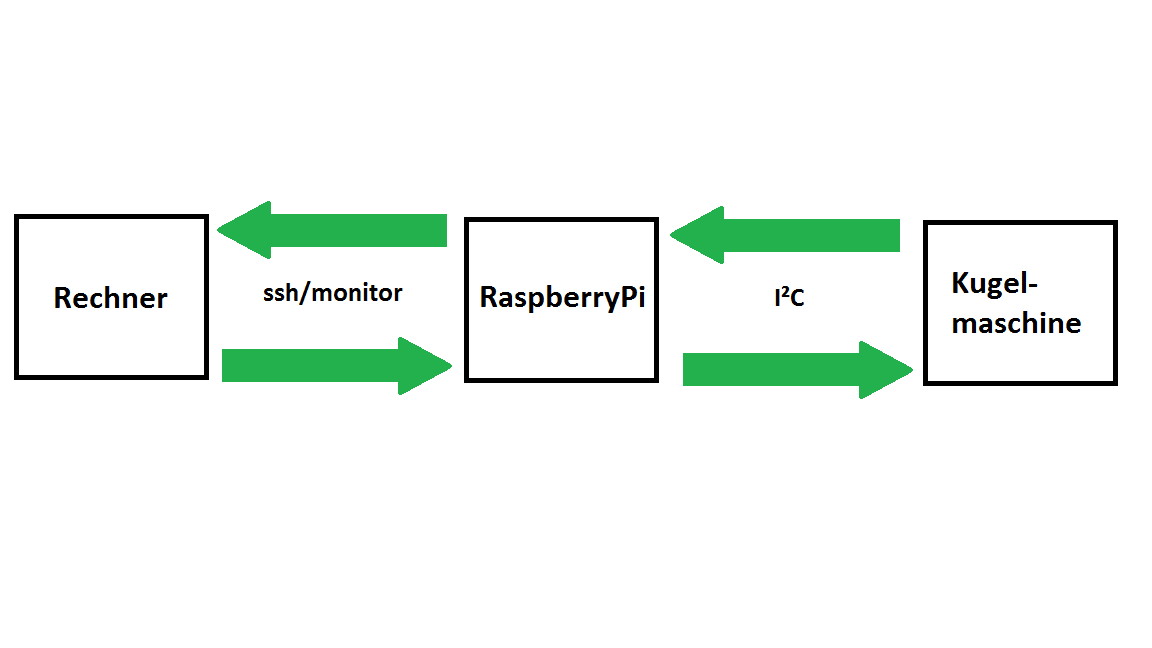
\includegraphics[width=15cm]{grafiken/Kommunitations_schema.png}
\caption{Kommunikationsschema}
\label{Kommunikationsschema}
\end{center}
\end{figure}
\noindent
Zunächst wurde versucht jedes einzelne Gerät (Motor, Lichtschranke, Klappen, Waage) der Kugelsortiermaschine anzusteuern.\\
Man konnte schnell erkennen, dass viele Semaphoren für die Sortierung nötig waren, da die Kugel immer nur weiter rollen darf, wenn der nächste Abschnitt, in den sie rollt, frei ist.
In Teilen des Programms musste C bzw. C++ Code verwendet werden, da manche Funktionen (z.B. Auslesen eines einzelnen Bits) noch nicht in OpenPEARL umgesetzt sind.\\
Beim Testen des Motors fiel auf, dass die analogen Werte sich ab einem bestimmten Durchmesser nicht mehr änderten.\\ 
Durch die Anpassung eines Wertes bei der Initialisierung des Analog-Digital-Converter(ADC) konnte dieser Fehler jedoch behoben werden.\\
\newpage

\subsection{Gerätesteuerung}
\subsubsection{Lichtschranken}
Die Kugelsortiermaschine besitzt insgesamt 9 Lichtschranken.\\
In unserer Anwendung sind die Lichtschranken so durchnummeriert, dass Lichtschranke 1 die oberste im Bau der Maschine ist und Lichtschranke 9 ganz unten links zu finden ist.\\
Die Nummern der Lichtschranken sind also von oben nach unten durchnummeriert.\\
Über den eingesetzten $I^2$C-Portexpander können aber nur maximal 8 Bit übertragen werden.
Deshalb erstellt man eine neue Variable “ls“ und hängt dem 8 Bit Block ein einzelnes Bit an.\\
\begin{lstlisting}
TAKE b8 FROM uls1_8;
TAKE b1 FROM uls9;
__cpp__('ls = _b1.bitCat(_b8);');
\end{lstlisting}
Somit enthält die Variable “ls“ den Status aller neun Lichtschranken.\\
Um aus dieser Variable den Wert einer Lichtschranke heraus zu lesen benötigt man wieder C-Code.\\
\begin{lstlisting}
DCL l1 BIT(1);
__cpp__('_l1 = _ls.getBit(9);');
\end{lstlisting}
In der Kugelsortieranwendung fragt der TASK readInputs alle 1/10 Sekunden die Werte der Lichtschranken neu ab.\\
\clearpage
\subsubsection{Dickenmessplatz}
Der Motor wird in der Kugelsortieranwendung dazu benutzt den Durchmesser einer Kugel zu bestimmen. Man kann ihm die drei Signale auf, zu oder stopp senden.\\
Des Weiteren kann man über zwei boolean Variablen auslesen, ob der Motor zu oder offen ist.\\
Da der Motor beim Zufahren nicht automatisch anhält wenn er geschlossen ist, sondern verklemmt, sorgte am Anfang für Verwirrung.\\
In der Sortieranwendung wird die Rolle des Motors im Task motor gemanaged.\\
Es gibt eine Variable Status die sich entweder im Zustand öffnend, schließend oder geschlossen befindet.\\
Um Verklemmung des Motors zu vermeiden wird die Polling-Methode mit kurzen Wartepausen(100ms) angewendet.\\
Das bedeutet es wird so lang in kurzen Zeitintervallen abgefragt ob der Motor offen bzw. geschlossen ist, bis das Ereignis zutrifft.\\
\newpage

\subsubsection{Klappen}
Insgesamt besitzt die Kugelsortiermaschine 7 Klappen bzw. Stoßer.\\
Um eine einzelne Klappe anzusprechen hätte wieder C-Code eingefügt werden müssen, doch dies war für unsere Anwendung nicht nötig.\\
Somit wurden immer auf alle Klappen geschrieben um sie auf oder zu zumachen.\\ 
Wie die Lichtschranken auch wurden die Klappen für unser Programm von oben nach unten durchnummeriert, sodass Klappe1 ganz oben und Klappe7 ganz unten links liegt.\\
Um zum Beispiel Klappe1 zu öffnen wurde das Bit 0000001 auf uhm1-7 gesendet.\\
\begin{lstlisting}
DCL (k1,allOff) BIT(7) INIT('0000001'B1, '0000000'B1);
SEND k1 TO uhm1_7;
AFTER 1 SEC RESUME;
SEND allOff TO uhm1_7;
\end{lstlisting}
Will man zwei Klappen gleichzeitig öffnen benötigte man jediglich ein anderes Bitmuser.\\
Zum Beispiel Klappe1 und Klappe2 :
\begin{lstlisting}
DCL test BIT(7) INIT('0000011' B1);
\end{lstlisting}
\subsubsection{Waage}
Genauso wie der Motor liefert die Waage in unserer Anwendung den analogen Wert für das Gewicht der Kugeln in Gramm.\\
Nachdem die Dichte ausgerechnet wurde, wird die Kugel von der Waage weggestoßen und je nach Dichte eine unterschiedliche Klappe geöffnet.\\
Das \nameref{Sortierkriterium} und die \nameref{Umrechnung analoger Werte} befinden sich in späteren Kapiteln.\\
\clearpage

\subsection{Sortierkriterium}\label{Sortierkriterium}
Anfangs war das Sortierkriterium ausschließlich der Wert der Dichte.\\
Doch bei Tests stellte sich heraus, dass die Klappe ganz rechts(Draufsicht) sich nicht vollständig öffnen ließ.\\ 
Wahrscheinlich weil die Maschine lange nicht in Benutzung war.\\
Es stellte sich jedoch heraus, dass kleine Kugeln dennoch durch die Öffnung passten.\\
Deshalb änderten wir das Sortierkriterium um jede Klappe auszunutzen.\\
Eine Kugel fällt in die 1. Schiene (Draufsicht ganz rechts), wenn ihr Durchmesser kleiner als 1.5cm ist.\\
Ist die Dichte einer Kugel kleiner 1 g/$cm^3$ wird sie in die 2. Schiene (Draufsicht eins weiter links) sortiert.\\
Eine Kugel fällt in die 3. Schiene, wenn ihre Dichte kleiner 2 g/$cm^3$ und größer 1 g/$cm^3$ ist.\\
In die 4. Schiene fällt eine Kugel mit einer Dichte kleiner 4 g/$cm^3$ und größer 2 g/$cm^3$.\\
Hat eine Kugel eine Dichte größer 4 g/$cm^3$ fällt sie in die 5. Schiene.\\ 
\newpage

\subsection{Umrechnung analoger Werte}\label{Umrechnung analoger Werte}
In der TASK rechner wird die Dichte der Kugel berechnet.\\
Um die Dichte auszurechnen benötigt man das Volumen und für das Volumen benötigt man den Durchmesser und das Gewicht der Kugel.\\
Die Machine liefert nur einen analogen Wert.\\
Das bedeutet man muss aus dem analogen Wert den realen Wert errechnen.\\
\\
In eine Excel Tabelle wurden die Analogen und realen Werte Aufgeschrieben, und der Faktor errechnet.\\
Zum Schluss wurde für das Gewicht und dem Durchmesser ein Durchschnittsfaktor errechnet.\\
\begin{figure}[h]
\begin{center}
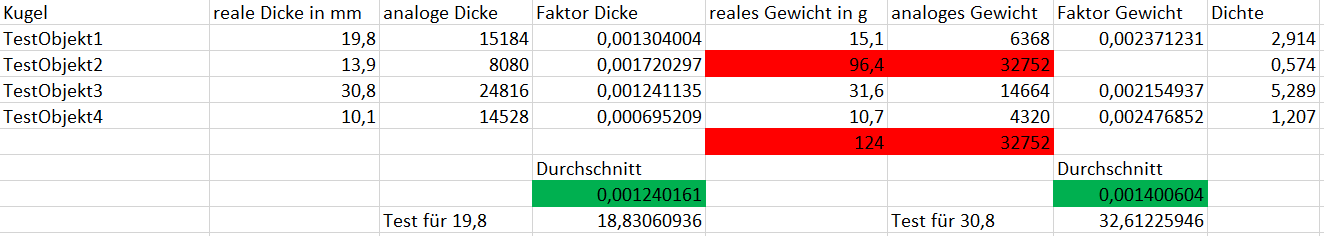
\includegraphics[width=15cm]{grafiken/UmrechnungsTabelle.png}
\caption{Umrechnung - Tabelle}
\label{Umrechnung}
\end{center}
\end{figure}
\\
Ein Wert für das Gewicht konnten wir nicht nutzen, da das analoge Gewicht ab einem bestimmten Gewicht gleich groß blieb.\\
Am Ende wurde mit den neuen Faktoren die Dichte von ein paar Kugeln berechnet.\\
\begin{figure}[h]
\begin{center}
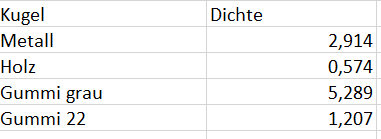
\includegraphics[width=10cm]{grafiken/UmrechnungTests.png}
\caption{Umrechnung - Tests}
\label{Umrechnung}
\end{center}
\end{figure}
\newpage




\subsection{Programmfluss}
Der Programmfluss wird durch 14 Semaphoren geregelt.\\
Um dies zu veranschaulichen ist im Anhang ein \nameref{Aktivitätsdiagramm} beigelegt.\\
In diesem ist jede Semaphore unterschiedlich eingefärbt, damit gleiche Semaphoren in unterschiedlichen Tasks besser erkennbar sind.\\
\\
Das Programm besteht aus 6 Tasks.\\
Die Main Task dumpInputs aktiviert die anderen 5 Tasks und kümmert sich anschließend nur noch um die Ausgabe.\\
\\
Der Task motor regelt den Zugriff zum Durchmesser lesen.\\
Bevor der Durchmesser gelesen werden darf, fordert der Task die Semaphoren motorgo und durchmesserlesen an.\\
Die semaphore motorgo prüft ob sich der Wert der Lichtschranke vor dem Motor geändert hat.\\
Falls ja wird sie auf true gesetzt.\\
Die Semaphore durchmesserlesen prüft ob die letzte Kugel von der Waage gestoßen wurde.\\
Sie wird beim Starten des Programms mit true initialisiert und sonst beim stoßen von der Waage befreit.\\
Nachdem der analoge Durchmesserwert gelesen wurde, wird die Semaphore mesdu befreit.\\
Sie bewirkt, dass im Task rechner aus dem analogen Wert der reale Durchmesser berechnet werden darf.\\
Anschließend wird die Semaphore waagefrei angefordert um sicher zu gehen, dass sich auf der Waage keine Kugel mehr befindet.\\
Zuletzt wird die Semaphore beginn freigeben, was dazu führt, dass wieder eine neue Kugel vom Start gestoßen werden kann.\\
Zudem wird die Semaphore Motorklappe freigegeben, damit nicht gleichzeitig auf unterschiedliche Klappen zugegriffen werden kann.\\
\\
Die Klasse readinputs kümmert sich um das einlesen der Lichtschranken.\\
Sie befreit die Semaphore motorgo, wenn sich der Wert der Lichtschranke vor dem Motor ändert.\\
Des weiteren bestätigt der Task das Sortieren, da sie die Lichtschranken in der Sortierrinne abfrägt.\\
\\
Der Task stoßer ist für die Steuerung der Waage verantwortlich.\\
Sobald der analoge Gewichtswert genommen wurde, wird die Semaphore mesgew befreit, sodass im Task rechner das reale Gewicht berechnet werden kann.\\
Danach wird die Semaphore stossen verlangt, welche nach dem errechne der Dichte der Kugel freigegeben wird.\\
Nachdem die Kugel weggestoßen wurde, wird die Semaphore durchmesserlesen befreit, sodass der Durchmesser der nächsten Kugel gelesen werden kann.\\
Sobald die Kugel in der richtigen Sortierrinne gelandet ist und an der Lichtschranke der Sortierrinne vorbeigerollt ist, schließen sich wieder alle Klappen.\\
Zuletzt wird die Semaphore waagefrei released, damit die nächste Kugel in die Waage rollen kann.\\
\\
Der Task rechner kümmert sich jeweils nur darum den realen Durchmesser,Gewicht und Dichte zu berechnen.\\
Er wartet durch Semaphoren darauf, dass neue analoge Werte geliefert werden und rechnet diese dann um.\\
\\
Der gesamte \nameref{Quellecode} des Programms befindet sich in unserem Repository.\\ 
\newpage




\subsection{Ausgabe}
Um den Kontrollfluss besser nachvollziehen zu können wurde eine Ausgabe entwickelt.
Die Komplette Ausgabe baut auf den Steuerzeichen der vt100 Konsole auf.\\
In der Main Task wird gleich zu Beginn ein Schema aufgebaut, dass sich danach nur bei Änderung ändert.
Diese zeigt die wichtigsten Daten in einer Tabelle an.\\
Wie zum Beispiel den ungefähren Aufenthalt der Kugel und enthält die Dichte der bisher sortierten Kugeln.\\
Auf der linken Seite der Ausgabe befindet sich die Tabelle.\\
\begin{figure}[h]
\begin{center}
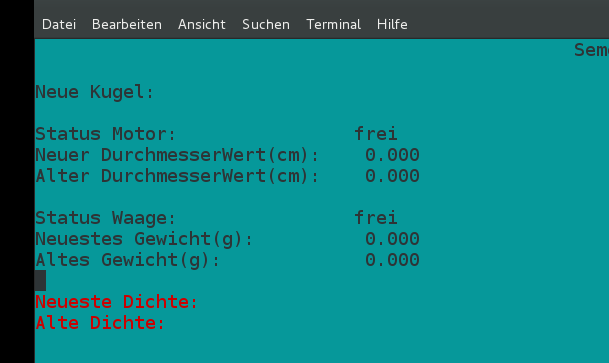
\includegraphics[width=10cm]{grafiken/Ausgabe_tabelle.png}
\caption{Ausgabe - Tabelle}
\label{Ausgabe}
\end{center}
\end{figure}
Sie enthält den Status, ob eine neue Kugel eingefügt werden kann, ob der Motor und Waage frei sind oder nicht, den Wert des letzten Durchmessers, Gewicht, und Dichte, den Wert des neuen Durchmessers, Gewicht und Dichte.
\newpage
\noindent
Auf der rechten Seite der Ausgabe befindet sich ein Schema der Maschine.
\begin{figure}[h]
\begin{center}
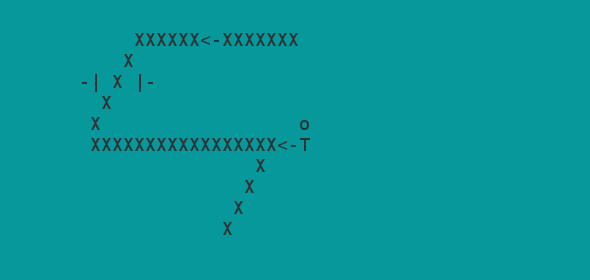
\includegraphics[width=10cm]{grafiken/Ausgabe_Schema.png}
\caption{Ausgabe - Schema}
\label{Ausgabe}
\end{center}
\end{figure}
Die X'se stellen den Weg der Kugelsortiermaschine dar.\\
Das Zeichen '<-' stellt den Stoßer ganz am Anfang der Kugelsortierung dar.\\
Durch das Zeichen '-| X |-' soll der Motor dargestellt werden.\\
Und das Zeichen 'T' soll die Waage symbolisieren.\\
Falls die Kugel sich an einem bestimmten Punkt in der Sortierung befindet, wird das X durch einen roten Kreis ersetzt.\\
\begin{figure}[h]
\begin{center}
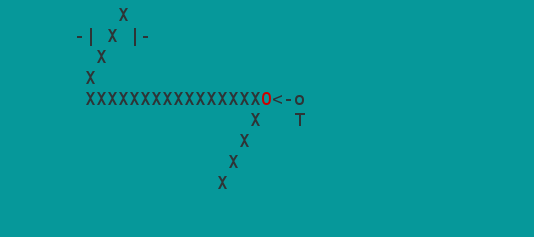
\includegraphics[width=10cm]{grafiken/Ausgabe_KugelinWaage.png}
\caption{Ausgabe - Waage}
\label{Ausgabe}
\end{center}
\end{figure}
\newpage
\noindent
Ganz unten in der Ausgabe befindet sich wieder eine Tabelle mit 5 Spalten.
Diese 5 Spalten symbolisieren die Rinnen in denen Die Kugel sortiert wird.
\begin{figure}[h]
\begin{center}

\includegraphics[width=14cm]{grafiken/Ausgabe_sortierte.png}
\caption{Ausgabe - Sortierung}
\label{Ausgabe}
\end{center}
\end{figure}
Der Kreis soll eine Kugel darstellen und daneben ist die Dichte angegeben mit der die Kugel sortiert wurde.
Die Werte der Kugeln stapeln sich in der Tabelle untereinander auf, so wie sie es auch in der Kugelsortiermaschine machen. 
\newpage

\subsection{Mögliche Verbesserungsansätze der Anwendung}
Die Anwendung besitzt keine Fehlerbehandlung und auch die Ausgabe ist noch verbesserungswürdig.\\
Wenn zum Beispiel keine Kugel im Motor ankommt fährt dieser trotzdem zu und das Programm geht weiter.\\
Man müsste in diesem Fall das Programm anhalten und wieder zurücksetzten.\\
Genauso ist es ein Fehler, wenn die Kugel irgendwo hängen bleibt oder einfach nicht weiter rollt.\\
Hierzu könnte man nach jeder Lichtschranke oder zumindest an den kritischen Stellen nach einer bestimmten Zeitüberschreitung, einen Fehler ausgeben.\\
Diese ganze Fehlerbehandlung könnte dann noch in die Ausgabe eingebaut werden, damit Fehler sofort erkannt werden und behoben werden können.\\
Auch der Zugriff auf die Klappen ist noch nicht optimal, da immer auf alle Klappen zugegriffen wird.\\
Sicherer wäre es immer nur einzelne Klappen anzusprechen.\\
In unserer Anwendung wurden Semaphoren benutzt um zu verhindern, dass gleichzeitig auf unterschiedliche Klappen zugegriffen wird.\\
Diese Semaphoren würden dadurch entfallen und den Programmfluss einfacher gestalten.\\  







